\subsection{Processamento digital de sinais analógicos}

\begin{frame}%[allowframebreaks]
  \frametitle{Processamento digital de sinais analógicos}
  \begin{figure}[h!]
  \centering
  \includegraphics[width=0.9\textwidth]{images/oppenheim_fig441.png}
  \caption{Processamento digital de sinais analógicos \citep{oppenheim2009}.}
  \label{fig:oppenheim_fig441}
  \end{figure}
  \bibentry{oppenheim2009}
\end{frame}
\note{
   Na prática temos que, 
   \begin{itemize}
   \item os sinais contínuos não são estritamente limitados em frequência;
   \item filtros ideais não são realizáveis;
   \item os conversores ideais C/D e D/C são aproximações de conversores A/D (analógico-digital)
        e D/A (digital-analógico).
   \end{itemize}
}
\note{
Devemos utilizar um filtro \textit{anti-aliasing}.

\begin{itemize}
\item usualmente é desejável utilizar uma taxa de amostragem baixa;
\item o próprio sinal e/ou ruído podem aparecer falseados como informação de baixa frequência;
\end{itemize}
}


\begin{frame}%[allowframebreaks]
  \frametitle{Filtro \textit{antialiasing} ideal}
  Resposta em frequência de um filtro \textit{antialiasing} ideal:
  \begin{equation}
  H_{\textmd{aa}} ( j \Omega ) = \begin{cases}1 \quad &, \vert \Omega \vert < \Omega_c < \pi/T ,\\ 
                                   0 &, \vert \Omega \vert > \Omega_c \textmd{.} 
			\end{cases}
  \end{equation}
\end{frame}


\begin{frame}[allowframebreaks]
  \frametitle{Processamento digital de sinais analógicos}

  \begin{figure}[h!]
  \centering
  \includegraphics[width=0.8\textwidth]{images/oppenheim_fig442.png}
  \caption{Processamento digital de sinais analógicos \citep{oppenheim2009}.}
  \label{fig:oppenheim_fig442}
  \end{figure}

  \bibentry{oppenheim2009}

  Considerando a entrada $x_a(t)$ e a saída $y_r(t)$, o sistema todo (compreendido entre entrada e saída) 
  pode ser visto como um sistema linear invariante no tempo com resposta $H (e^{j \Omega T})$.

  Assim, a resposta total do sistema será
  \begin{equation}
  H_{\text{eff}} (j \Omega) \approx H_{aa} (j \Omega) H (e^{j \Omega T}) \textmd{,}
  \end{equation}
  ou seja,
  \begin{equation}
    H_{\text{eff}} (j \Omega) \approx \begin{cases} H(e^{j\Omega T}) \quad &, \vert \Omega \vert < \Omega_c,\\ 
                                   0 &, \vert \Omega \vert > \Omega_c \textmd{.} \end{cases}
  \end{equation}
  Na prática, teremos a aproximação acima pois 
  a resposta em frequência de $H_{\text{aa}} (j \Omega)$ não é idealmente limitada em frequência,
  mas podemos fazer $H_{\text{aa}} (j \Omega)$ pequeno para $\vert \Omega \vert > \pi / T$, minimizando assim 
  o \textit{aliasing}.
\end{frame} 
\note{
  Filtros abruptos são de difícil implementação e alto custo. Além disso, geralmente possuem resposta
  em fase altamente não-linear.
  Para que o sistema opere com
  diferentes taxas de amostragem, devemos ter filtros ajustáveis.
} 

\begin{frame}[allowframebreaks]
  \frametitle{Utilizando uma conversão A/D com sobre-amostragem para simplificar o filtro analógico \textit{antialiasing}}

  \begin{figure}[h!]
  \centering
  \includegraphics[width=0.6\textwidth]{images/oppenheim_fig443.png}
  \caption{Utilizando uma conversão A/D com sobre-amostragem para simplificar o filtro analógico \textit{antialiasing} \citep{oppenheim2009}.}
  \label{fig:oppenheim_fig443}
  \end{figure}
  \bibentry{oppenheim2009}

  \begin{description}
  \item[$\Omega_N$]: frequência mais alta que desejamos manter
  \item[$M$]: fator de sobre-amostragem
  \end{description}

\end{frame}


\begin{frame}[allowframebreaks]
  \frametitle{Sobre-amostragem e decimação}

  \begin{figure}[h!]
  \centering
  \includegraphics[width=0.35\textwidth]{images/oppenheim_fig444.png}
  \caption{Exemplo \citep{oppenheim2009}}
  \label{fig:oppenheim_fig444}
  \end{figure}
  %{\small \bibentry{oppenheim2009}}

  \begin{figure}[h!]
  \centering
  \includegraphics[width=0.8\textwidth]{images/oppenheim_fig444ab.png}
  %\caption{}
  \label{fig:oppenheim_fig444ab}
  \end{figure}

  \begin{figure}[h!]
  \centering
  \includegraphics[width=0.8\textwidth]{images/oppenheim_fig444cd.png}
  %\caption{}
  \label{fig:oppenheim_fig444cd}
  \end{figure}

\end{frame}


\begin{frame}%[allowframebreaks]
  \frametitle{Configuração física para conversão analógico-digital}

  \begin{figure}[h!]
  \centering
  \includegraphics[width=0.6\textwidth]{images/oppenheim_fig445.png}
  \caption{Configuração física para conversão analógico-digital \citep{oppenheim2009}.}
  \label{fig:oppenheim_fig445}
  \end{figure}

  \begin{description}
  \item[$x_a(t)$]: sinal analógico
  \item[{$\hat{x}_{B}[n]$}]: sinal digital (amostrado e quantizado)
  \item[$T$]: período de amostragem
  \end{description}

\end{frame}


\begin{frame}[allowframebreaks]
  \frametitle{Representação de um \textit{sample-and-hold} ideal}

  \hvFloat[floatPos=htb,capPos=right,capVPos=bottom,objectPos=c]{figure}{\includegraphics[width=0.45\textwidth]{images/oppenheim_fig446.png}}
  {Sample-and-hold \citep{oppenheim2009}.}{fig:oppenheim_fig446}

  A saída de um \textit{sample-and-hold} ideal é dada por
  \begin{equation}
  x_0(t) = \sum_{n=-\infty}^{\infty} x[n] h_0 (t -nT)
  \label{eq:x0t}
  \end{equation}
  onde $x[n] = x_a(nT)$ são as amostras ideais (não quantizadas) de $x_a(t)$ e 
  $h_0(t)$ é a resposta ao impulso do \textit{hold} de ordem zero, i.e.,
  %where $x[n] = x_a(nT)$ are the ideal samples of $x_a(t)$ and $h_0(t)$ is the impulse response of the zero-order-hold system, i.e.,
  \begin{equation}
  h_0(t) = \begin{cases} 1  \quad &,  0 < t < T ,\\ 
                         0 &, \mbox{caso contrário.}\end{cases} 
  \end{equation}
  A Equação \ref{eq:x0t} é equivalente a
  %The Equation \ref{eq:x0t} has the equivalent form
  \begin{equation}
  x_0(t) = h_0(t) \ast \sum_{n=-\infty}^{\infty} x_a(nT) \delta(t-nT) \textmd{ . }
  \end{equation}
\end{frame}
\note{
O circuito de uma \textit{sample-and-hold} é projetado para amostrar $x_a(t)$ `instantaneamente'
e `manter' o valor da amostra constante até que a próxima amostra seja tomada. Isto é necessário
para fornecer uma tensão de entrada constante no conversor A/D.
}

\begin{frame}%[allowframebreaks]
  \frametitle{Equivalência Conceitual}
  O sistema composto pelo \textit{sample-and-hold} seguido por um conversor A/D
  \begin{figure}[h!]
  \centering
  \includegraphics[width=0.4\textwidth]{images/oppenheim_fig445.png}
  %\caption{}
  \label{fig:oppenheim_fig445_2}
  \end{figure}
  é equivalente ao seguinte sistema, composto por um conversor C/D ideal seguido por um quantizador
  \begin{figure}[h!]
  \centering
  \includegraphics[width=0.6\textwidth]{images/oppenheim_fig447.png}
  \caption{Sistema equivalente \citep{oppenheim2009}.}
  \label{fig:oppenheim_fig447}
  \end{figure}
\end{frame}

\begin{frame}[allowframebreaks]
  \frametitle{Quantizador Uniforme}
  Um quantizador é um sistema não-linear cuja operação é definida por uma função $Q(\cdot)$,
  \begin{equation}
  \hat{x}[n] = Q(x[n]) .
  \end{equation}

  \framebreak

  \hvFloat[floatPos=htb,capPos=right,capVPos=bottom,objectPos=c]{figure}{\includegraphics[width=0.7\textwidth]{images/oppenheim_fig448.png}}
  {Quantizador uniforme de 3 bits \citep{oppenheim2009}.}{fig:oppenheim_fig448}


%  \begin{figure}[h!]
%  \centering
%  \includegraphics[width=0.7\textwidth]{/home/leoca/ee/ufsj/2014_01/audiovideo/aula/images/oppenheim_fig448.png}
%  \caption{Quantizador uniforme de 3 bits \citep{oppenheim2009}.}
%  \label{fig:oppenheim_fig448}
%  \end{figure}

  \framebreak

  O bit mais à esquerda, o bit mais significativo, é considerado o bit de sinal. 
  Os demais bits representam na forma binária uma fração (ou inteiro).
  \begin{figure}[h!]
  \centering
  \includegraphics[width=0.4\textwidth]{images/oppenheim_tab_bincode.png}
  \caption{Código binário: complemento de dois \citep{oppenheim2009}.}
  \label{fig:oppenheim_tab_bincode}
  \end{figure}
  De forma geral, temos $(B+1)$-bits, complemento de 2 de uma fração binária na forma 
  $a_0 . a_1 a_2 \ldots a_B$, cujo valor é
  \begin{equation}
  -a_0 2^0 + a_1 2^{-1} + a_2 2^{-2} + \cdots + a_B 2^{-B} \textmd{ .}
  \end{equation}

  \framebreak

  \begin{description}
  \item[$X_m$]: estensão do sinal na entrada do conversor A/D
  \item[$\Delta$]: tamanho do passo do quantizador
  \item[$B+1$]: número de bits do quantizador
  \end{description}
 
  \begin{equation}
  \label{eq-Xm-B}
  \Delta = \frac{2 X_m}{2^{B+1}} = \frac{X_m}{2^B} \textmd{ .}
  \end{equation}

  A relação entre as palavras do quantizador e as amostras quantizadas é dada por
  \begin{equation}
  \hat{x}[n] = X_m \hat{x}_B [n] \textmd{ ,}
  \end{equation}
  pois assumimos que $\hat{x}_B [n]$ é um número binário $-1 \leq \hat{x}_B [n] < 1$ (complemento de dois).

  Para simplificar, podemos assumir que o sinal de entrada é normalizado.

\end{frame}

\begin{frame}[allowframebreaks]
  \frametitle{Erro de quantização} 

  O erro de quantização é definido por
  \begin{equation}
  e[n] = \hat{x} [n] - x[n] \textmd{ .}
  \end{equation}

  O erro de quantização satisfaz
  \begin{equation}
  \ \Delta/2 < e[n] \leq \Delta/2
  \end{equation}
  sempre que
  \begin{equation}
  (- X_m - \Delta/2) < x[n] \leq (X_m - \Delta/2) \textmd{ .}
  \end{equation}
  Se $x[n]$ estiver fora desta faixa, o erro de quantização será maior do que $\Delta/2$, e as amostras
  serão `grampeadas'.
\end{frame}

\begin{frame}[allowframebreaks]
  \frametitle{Modelo aditivo do erro de quantização}
  \begin{figure}[h!]
  \centering
  \includegraphics[width=0.4\textwidth]{images/oppenheim_fig450.png}
  \caption{Modelo aditivo do erro de quantização \citep{oppenheim2009}.}
  \label{fig:oppenheim_fig450}
  \end{figure}

  \vspace{-2ex}
  \begin{small}
  A representação estatística do erro de quantização é baseada nas seguintes suposições:
  \begin{itemize}
  \item $e[n]$ é um processo estocástico estacionário;
  \item $e[n]$ é descorrelacionada com $x[n]$;
  \item o erro é um ruído branco, suas amostras são descorrelacionadas
  \item a pdf do erro é uniforme 
  \end{itemize}
  \end{small}
  
  \framebreak

  Para $\Delta$ pequeno, podemos assumir que $e[n]$ é um ruído branco uniforme em $[-\Delta/2, \Delta/2]$.

  \begin{figure}[h!]
  \centering
  \includegraphics[width=0.55\textwidth]{images/oppenheim_fig452.png}
  \caption{Modelo do ruído \citep{oppenheim2009}.}
  \label{fig:oppenheim_fig452}
  \end{figure}

  \begin{description}
  \item[média]: $\mu_e = 0$;
  \item[variância]: $\sigma_e^2 = \Delta^2/12$.
  \end{description}

  \begin{equation}
  \sigma_e^2 = \int_{-\Delta/2}^{\Delta/2} e^2 \frac{1}{\Delta} de = \frac{\Delta^2}{12} \textmd{ .}
  \end{equation}

  Para um quantizador de $(B+1)$ bits e fundo de escala $X_m$, a variância do ruído (ou potência)
  será dada por
  \begin{equation}
  \sigma_e^2 = \frac{2^{-2B}X_m^2}{12} \textmd{ ,}
  \end{equation}
  onde $\Delta = X_m/2^B$.


  \framebreak

  A relação sinal-ruído de quantização para um quantizador com $(B+1)$ bits é
  \begin{eqnarray}
  \textmd{SQNR} &=& 10 \log_{10} \left( \frac{\sigma_x^2}{\sigma_e^2} \right) = 10 \log_{10} \left( \frac{12 \cdot 2^{2B} \sigma_x^2}{X_m^2} \right) \nonumber \\
      &=& 6.02 B + 10.8 - 20 \log_{10} \left( \frac{X_m}{\sigma_x} \right) \textmd{ .}
  \end{eqnarray}
  Aproximadamente 6dB para cada bit.

\end{frame} 


\subsection{Conversão discreto-contínuo}
\begin{frame}[allowframebreaks]
  \frametitle{Conversão discreto-contínuo}
  \begin{figure}[h!]
  \centering
  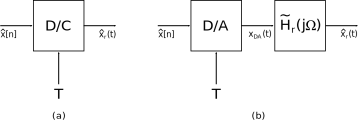
\includegraphics[width=0.8\textwidth]{images/da-conversion.pdf}
  \caption{Conversão discreto para contínuo.}
  \label{fig:da-conversion}
  \end{figure}

  \framebreak

  A reconstrução é representada por
  \begin{equation}
  X_r (j\Omega) = X(e^{j\Omega T}) H_r(j\Omega)
  \end{equation}
  onde $X(e^{j\Omega})$ é a transformada discreta de Fourier de $x[n]$ e $X_r(j\Omega)$
  é a transformada de Fourier do sinal reconstruído. O filtro de reconstrução ideal é dado por
  \begin{equation}
  H_r(j\Omega) = \begin{cases} T  \quad &, |\Omega|  < \pi/T ,\\ 0 &, |\Omega| > \pi/T \textmd{ .}\end{cases}
  \end{equation}
  A relação entre $x_r(t)$ e $x[n]$ será dada por
  \begin{equation}
  x_r (t) = \sum_{n=-\infty}^{\infty} x[n] \frac{\sin [\pi (t-nT)/T]}{\pi(t-nT)/T} \textmd{ .}
  \end{equation}

  \framebreak

  \begin{figure}[h!]
  \centering
  \includegraphics[width=0.5\textwidth]{images/oppenheim_fig453.png}
  \caption{Modelo do conversor D/A \citep{oppenheim2009}.}
  \label{fig:oppenheim_fig453}
  \end{figure}

  \begin{eqnarray}
  x_{\text{DA}}(t) &=& \sum_{n=-\infty}^{\infty} X_m \hat{x}_B[n] h_0(t-nT) \nonumber \\
            &=& \sum_{n=-\infty}^{\infty} \hat{x}[n] h_0(t-nT) \textmd{ .}
  \end{eqnarray}

  \framebreak

  Utilizando o modelo aditivo do ruído de quantização (ver \Cref{fig:oppenheim_fig450}),
  podemos considerar $x_{\text{DA}}(t)$ como composta em duas partes, uma devida ao sinal
  e outra devida ao ruído de quantização. Assim podemos analisar os efeitos da quantização.

  \begin{equation}
   x_{\text{DA}}(t) = \sum_{n=-\infty}^{\infty} x[n]h_0(t-nT) + \sum_{n=-\infty}^{\infty} e[n] h_0(t-nT) \textmd{ .}
  \end{equation}

  Definimos
  \begin{equation}
  \label{eq-x0t}
  x_0(t) = \sum_{n=-\infty}^{\infty} x[n]h_0(t-nT) \textmd{ , e}
  \end{equation}
  \begin{equation}
  \label{eq-e0t}
  e_0(t) = \sum_{n=-\infty}^{\infty} e[n] h_0(t-nT) \textmd{ ,}
  \end{equation}
  de forma que
  \begin{equation}
  x_{\text{DA}}(t) = x_0(t) + e_0(t) \textmd{ .}
  \end{equation}

  A transformada de Fourier da Equação \ref{eq-x0t} é
  \begin{eqnarray}
  X_0(j\Omega) &=& \sum_{n=-\infty}^{\infty} x[n] H_0(j\Omega) e^{-j \Omega nT} \nonumber \\
               &=& \left( \sum_{n=-\infty}^{\infty} x[n] e^{-j \Omega nT} \right) H_0(j\Omega) \nonumber \\
               &=& X(e^{j\Omega T}) H_0(j\Omega) \textmd{ .}
  \end{eqnarray}
  Como
  \vspace{-0.2cm}
  \begin{equation}
  X(e^{j\Omega T}) = \frac{1}{T} \sum_{k=-\infty}^{\infty} X_a \left( j \left( \Omega - \frac{2\pi k}{T} \right) \right) .
  \end{equation}
  segue que
  \vspace{-0.2cm}
  \begin{equation}
  \label{eq-X0jomega}
  X_0(j\Omega) = \left[  \frac{1}{T} \sum_{k=-\infty}^{\infty} X_a \left( j \left( \Omega - \frac{2\pi k}{T} \right) \right) \right] H_0(j\Omega) \textmd{ .}
  \end{equation}
\end{frame}

\begin{frame}[allowframebreaks]
  \frametitle{Filtro de Reconstrução}
  Se $X_a(j \Omega)$ é limitado em frequência abaixo de $\pi/T$,
  as cópias deslocadas de $X_a(j \Omega)$ não se sobrepõem na Equação \ref{eq-X0jomega},
  e se definirmos o filtro de reconstrução compensado como
  \begin{equation}
  \tilde{H}_r (j\Omega) = \frac{H_r (j\Omega)}{H_0(j \Omega)},
  \end{equation}
  então, a saída do filtro será $x_a(t)$ se a entrada for $x_0(t)$.
  A resposta em frequência do \textit{hold} de ordem zero é
  \begin{equation}
  H_0 (j\Omega) = \frac{2 \sin(\Omega T/2)}{\Omega} e^{-j\Omega T/2} .
  \end{equation}
  Desta forma, o filtro de reconstrução compensado é dado por
  \begin{equation}
  \tilde{H}_r (j\Omega) = \begin{cases}\frac{\Omega T/2}{\sin(\Omega T/2)} e^{j \Omega T /2} \quad & |\Omega| \leq \pi/T ,\\
                                     0 & |\Omega| > \pi/T .\end{cases}
  \end{equation}

  \begin{figure}[h!]
  \centering
  \includegraphics[width=0.8\textwidth]{images/oppenheim_fig454.png}
  \caption{Filtro de reconstrução compensando o efeito do hold \citep{oppenheim2009}.}
  \label{fig:oppenheim_fig454}
  \end{figure}

\end{frame}


\begin{frame}[allowframebreaks]
  \frametitle{Configuração física da conversão digital analógico}
  \begin{figure}[h!]
  \centering
  \includegraphics[width=0.5\textwidth]{images/oppenheim_fig455.png}
  \caption{Configuração física para a conversão digital-analógico \citep{oppenheim2009}.}
  \label{fig:oppenheim_fig455}
  \end{figure}

  \framebreak 
  O sinal reconstruído na saída é
  \begin{eqnarray}
  \hat{x}_r (t) &=& \sum_{n=-\infty}^{\infty} \hat{x}[n] \frac{\sin [\pi (t - nT)/T]}{\pi (t - nT)/T} \\
                &=& \sum_{n=-\infty}^{\infty} x[n] \frac{\sin [\pi (t - nT)/T]}{\pi (t - nT)/T} + 
                    \sum_{n=-\infty}^{\infty} e[n] \frac{\sin [\pi (t - nT)/T]}{\pi (t - nT)/T} . \nonumber
  \end{eqnarray}
  Ou seja, a saída é dada por 
  \begin{equation}
  \hat{x}_r (t) = x_a(t) + e_a(t),
  \end{equation}
  onde $e_a(t)$ é o ruído branco limitado em frequência.

\end{frame}


\begin{frame}[allowframebreaks]
  \frametitle{Sistema para processamento digital de sinais analógicos}
  %System for digital processing of analog signals}
  \begin{figure}[h!]
  \centering
  \includegraphics[width=\textwidth]{images/oppenheim_fig441b.png}
  \caption{Sistema para processamento digital de sinais analógicos \citep{oppenheim2009}.}
  \label{fig:oppenheim_fig441b}
  \end{figure}

  \begin{equation}
  \hat{y}_r (t) = y_a (t) + e_a (t)
  \end{equation}
  
  \begin{equation}
  Y_a(j\Omega) = \tilde{H}_r(j\Omega) H_0(j\Omega) H(e^{j\Omega T}) H_{\text{aa}}(j\Omega) X_c(j\Omega) 
  \end{equation}
  onde 
  \begin{itemize}
  \item $H_{\text{aa}}(j\Omega)$ filtro \textit{antialiasing}
  \item $H_0(j\Omega)$ \textit{hold} de ordem zero do conversor D/A 
  \item $\tilde{H}_r(j\Omega)$ filtro passa-baixas de reconstrução 
  \end{itemize}

  
  Assumindo que o ruído de quantização introduzido pelo conversor A/D é branco com
  variância $\sigma_e^2 = \Delta^2/12$, podemos mostrar que o espectro de densidade de potência do ruído na saída é
  \begin{equation}
  P_{e_a} (j\Omega) = \vert \tilde{H}_r(j\Omega) H_0(j\Omega) H(e^{j\Omega T}) \vert^2 \sigma_e^2 .
  \end{equation}
  A resposta em frequência efetiva total de $x_c(t)$ a $y_r(t)$ é
  \begin{equation}
  H_{\text{eff}}(j\Omega) = \tilde{H}_r(j\Omega) H_0(j\Omega) H(e^{j\Omega T}) H_{\text{aa}}(j\Omega) .
  \end{equation}
\end{frame}



%\begin{frame}%[allowframebreaks]
%  \frametitle{}
%\end{frame}

%\begin{frame}%[allowframebreaks]
%  \frametitle{}
%\end{frame}

%\begin{frame}%[allowframebreaks]
%  \frametitle{}
%\end{frame}


